% -------------------------------------------------------------------
% Build notes:
% Recommended engine: XeLaTeX (or LuaLaTeX) because this document uses fontspec
% Bibliography backend: biber (biblatex is configured in the class)
%
% Quick build (recommended, from this folder):
%   latexmk -pdf -xelatex -use-biber Main.tex
%
% Manual build sequence (if you don't use latexmk):
%   xelatex Main.tex
%   biber Main
%   xelatex Main.tex
%   xelatex Main.tex
%
% Fonts: project class expects THSarabun files in Class/Font/ or the system fonts.
% If compilation fails due to fonts, either install the THSarabun fonts system-wide
% or copy the font files into docs/special_project/Class/Font/ (see project_report.cls).
% -------------------------------------------------------------------
\documentclass{Class/project_report}
\setTHSarabunFont
\geometry{a4paper,top=1.5in,bottom=1in,left=1.5in,right=1in}
\pagestyle{plain} % ตั้งค่า pagestyle เริ่มต้น
\newcolumntype{L}{>{\RaggedRight\arraybackslash}X} 
\begin{document}

    % Setup for Figures (centered label and text)
    \captionsetup[figure]{
      font={normalsize},
      labelfont={bold16pt},
      labelsep=quad,
      justification=centering,
      singlelinecheck=false,
      name={ภาพที่} % Add this line
    }
    % Setup for Tables (raggedright label and text)
    \captionsetup[table]{
      font={normalsize},
      labelfont={bold16pt},
      labelsep=quad,
      justification=raggedright,
      singlelinecheck=false,
      name={ตารางที่} % Add this line
    }
    \input{Project_000_Cover}

    
    \input{Project_001_Certificate1} %กรณี ไม่มี ที่ปรึกษาร่วม
    %\input{Project_001_Certificate2} %กรณี มี ที่ปรึกษาร่วม

    
    \newpage
    \thaiPageStyle
    \setcounter{page}{1}
    \fontSixTeen
    \justifying
    \input{Project_002_Abstract}
    \newgeometry{a4paper,top=1.5in,bottom=1in,left=1.5in,right=1in,includehead}
    \setTHSarabunFont
    \fontsize{16}{16}\selectfont
    \thaiPageStyle
    \customTOCthai
    \newpage
    \customLOFthai
    \newpage
    \customLOTthai
    \clearpage % ขึ้นหน้าใหม่หลังจากหน้าที่มีการปรับ margin
    \restoregeometry % คืนค่า geometry กลับเป็นค่าเริ่มต้น
    \fancyhf{} % ล้างการตั้งค่า fancyhdr ของหน้าที่ปรับ
    \setTHSarabunFont
    \fontsize{16}{16}\selectfont
    \thaiPageStyle
    
    \newpage
    \setlength{\headheight}{0cm}
    \setcounter{page}{1}
    \arabicPageTopRight % ตั้งค่าต่อไปใช้สไตล์อารบิกมุมขวาบน
    \customTOCarabic
    \input{Project_010_Chapter1}
    \input{Project_020_Chapter2}
    %*************************************
% บทที่ 3
%*************************************
\chapterTitle{3}{วิธีการดำเนินงานและการออกแบบระบบ}

% Project Methodology
\section{ขั้นตอนการดำเนินงาน}

\hspace*{1.5em} %ย่อหน้า
การพัฒนาแพลตฟอร์มคลัสเตอร์เสมือนสำหรับการศึกษามีขั้นตอนการดำเนินงานที่เป็นระบบ โดยแบ่งออกเป็น 5 ขั้นตอนหลัก ดังนี้

\begin{mycustomenum2}
    \item \textbf{การศึกษาและวิเคราะห์ความต้องการ} การสำรวจความต้องการของผู้ใช้งาน การศึกษาระบบที่มีอยู่เดิม และการกำหนดข้อกำหนดของระบบ
    \item \textbf{การออกแบบสถาปัตยกรรมระบบ} การออกแบบโครงสร้างระบบทั้งหมด การเลือกเทคโนโลยีที่เหมาะสม และการออกแบบฐานข้อมูล
    \item \textbf{การพัฒนาระบบ} การพัฒนาส่วนต่าง ๆ ของระบบตามสถาปัตยกรรมที่ออกแบบไว้
    \item \textbf{การทดสอบระบบ} การทดสอบการทำงานของระบบ การทดสอบประสิทธิภาพ และการทดสอบความปลอดภัย
    \item \textbf{การประเมินผลและปรับปรุง} การประเมินผลการใช้งานจริง และการปรับปรุงระบบตามผลการประเมิน
\end{mycustomenum2}

% Research and Requirements Analysis
\section{การศึกษาและวิเคราะห์ความต้องการ}

% 3.2.1
\subsection{การสำรวจความต้องการผู้ใช้งาน}

\hspace*{1.5em} %ย่อหน้า
ผู้จัดทำได้ดำเนินการสำรวจความต้องการจากกลุ่มผู้ใช้งานในภาควิชาเทคโนโลยีสารสนเทศ ได้แก่

\begin{mycustomitem}
    \item \textbf{อาจารย์} ต้องการระบบจัดการเครื่องเสมือนที่ใช้งานง่าย สำหรับการสอนและการวิจัย
    \item \textbf{นักศึกษา} ต้องการเข้าถึงเครื่องเสมือนสำหรับการเรียนและทำโครงงาน
    \item \textbf{ผู้ดูแลระบบ} ต้องการเครื่องมือติดตามและจัดการระบบที่มีประสิทธิภาพ
\end{mycustomitem}

% 3.2.2
\subsection{การวิเคราะห์ระบบเดิม}

\hspace*{1.5em} %ย่อหน้า
จากการศึกษาระบบที่มีอยู่เดิม พบปัญหาและข้อจำกัดดังนี้

\begin{mycustomitem}
    \item \textbf{การใช้งานที่ซับซ้อน} ต้องใช้ความรู้ทางเทคนิคสูงในการจัดการเครื่องเสมือน
    \item \textbf{ขาดระบบจัดการผู้ใช้} ไม่มีการแยกสิทธิ์การใช้งานตามบทบาท
    \item \textbf{ประสิทธิภาพต่ำ} การสร้างและลบเครื่องเสมือนใช้เวลานาน
    \item \textbf{ขาดการติดตาม} ไม่มีระบบ Monitoring การใช้ทรัพยากร
\end{mycustomitem}

% 3.2.3
\subsection{ข้อกำหนดของระบบ}

\hspace*{1.5em} %ย่อหน้า
จากการวิเคราะห์ความต้องการ ได้กำหนดข้อกำหนดของระบบดังนี้

\hspace*{1.5em} %ย่อหน้า
\textbf{ข้อกำหนดเชิงหน้าที่ (Functional Requirements)}
\begin{mycustomitem}
    \item ระบบต้องสามารถสร้าง แก้ไข และลบเครื่องเสมือนได้
    \item ระบบต้องรองรับการจัดการผู้ใช้แบบ Role-Based Access Control
    \item ระบบต้องมีระบบยืนยันตัวตนผ่าน OAuth 2.0
    \item ระบบต้องสามารถติดตามการใช้ทรัพยากรแบบ Real-time
    \item ระบบต้องส่งการแจ้งเตือนเมื่อมีการเปลี่ยนแปลงสถานะ
\end{mycustomitem}

\hspace*{1.5em} %ย่อหน้า
\textbf{ข้อกำหนดที่ไม่เกี่ยวกับหน้าที่ (Non-Functional Requirements)}
\begin{mycustomitem}
    \item \textbf{ประสิทธิภาพ} การสร้างเครื่องเสมือนต้องใช้เวลาไม่เกิน 3 นาที
    \item \textbf{ความพร้อมใช้งาน} ระบบต้องพร้อมใช้งานอย่างน้อย 99.5% ของเวลา
    \item \textbf{ความปลอดภัย} ข้อมูลต้องได้รับการเข้ารหัสและจัดเก็บอย่างปลอดภัย
    \item \textbf{ความยืดหยุ่น} ระบบต้องรองรับการขยายทรัพยากรได้ในอนาคต
\end{mycustomitem}

% System Architecture Design
\section{การออกแบบสถาปัตยกรรมระบบ}

% 3.3.1
\subsection{สถาปัตยกรรมระบบโดยรวม}

\begin{figure}[htbp]
    \centering
    
\includegraphics[width=1.0\textwidth]{Image/web/context_diagram.png}
    \caption{แผนภาพบริบทของระบบแพลตฟอร์มคลัสเตอร์เสมือน}
    \label{fig:context_diagram}
\end{figure}

\hspace*{1.5em} %ย่อหน้า
ระบบแพลตฟอร์มคลัสเตอร์เสมือนได้รับการออกแบบในรูปแบบ Microservices Architecture โดยแบ่งเป็นส่วนประกอบหลัก 3 ส่วน คือ

\begin{mycustomitem}
    \item \textbf{Frontend} เว็บแอปพลิเคชันสำหรับผู้ใช้งาน พัฒนาด้วย Next.js และ React
    \item \textbf{Backend} เซิร์ฟเวอร์ API สำหรับการจัดการข้อมูลและการยืนยันตัวตน พัฒนาด้วย Elysia.js
    \item \textbf{Instance Management} เซอร์วิสจัดการเครื่องเสมือนและการสื่อสารกับ Proxmox VE
\end{mycustomitem}

\hspace*{1.5em} %ย่อหน้า
จากภาพที่ \ref{fig:context_diagram} แผนภาพบริบทข้างต้นแสดงให้เห็นถึงการเชื่อมต่อและการสื่อสารระหว่างส่วนประกอบต่าง ๆ ของระบบ โดยผู้ใช้งานสามารถเข้าถึงระบบผ่านเว็บแอปพลิเคชัน ที่จะสื่อสารกับ Backend API และระบบจัดการเครื่องเสมือนเพื่อให้บริการที่สมบูรณ์

% 3.3.2
\subsection{การออกแบบฐานข้อมูล}

\hspace*{1.5em} %ย่อหน้า
ระบบใช้ PostgreSQL เป็นฐานข้อมูลหลัก โดยออกแบบตารางหลักดังนี้

\begin{mycustomitem}
    \item \textbf{User Table} เก็บข้อมูลผู้ใช้งาน บทบาท และสิทธิ์การเข้าถึง
    \item \textbf{Instance Table} เก็บข้อมูลเครื่องเสมือน การกำหนดค่า และสถานะ
    \item \textbf{Template Table} เก็บข้อมูล Template สำหรับการสร้างเครื่องเสมือน
    \item \textbf{Activity Log Table} เก็บประวัติการใช้งานและการเปลี่ยนแปลง
    \item \textbf{Resource Usage Table} เก็บข้อมูลการใช้ทรัพยากรแบบ Time-series
\end{mycustomitem}

% 3.3.3
\subsection{การออกแบบ API และการสื่อสาร}

\hspace*{1.5em} %ย่อหน้า
ระบบใช้ RESTful API เป็นหลักในการสื่อสารระหว่างส่วนประกอบต่าง ๆ โดยมีการออกแบบดังนี้

\begin{mycustomitem}
    \item \textbf{Authentication Endpoints} สำหรับการ Login, Logout และ Token Management
    \item \textbf{Instance Management Endpoints} สำหรับการจัดการเครื่องเสมือน (CRUD Operations)
    \item \textbf{Monitoring Endpoints} สำหรับการติดตามการใช้ทรัพยากร
\end{mycustomitem}

% 3.3.4
\subsection{การออกแบบระบบ Message Queue}

\hspace*{1.5em} %ย่อหน้า
เพื่อรองรับการประมวลผลแบบ Asynchronous ระบบใช้ RabbitMQ เป็น Message Broker โดยออกแบบ Queue หลักดังนี้

\begin{mycustomitem}
    \item \textbf{Instance Creation Queue} สำหรับงานการสร้างเครื่องเสมือน
    \item \textbf{Instance Deletion Queue} สำหรับงานการลบเครื่องเสมือน
\end{mycustomitem}

% Tools and Technologies Used
\section{เครื่องมือและเทคโนโลยีที่ใช้ในการพัฒนา}

% 3.4.1
\subsection{เทคโนโลยี Frontend}

\hspace*{1.5em} %ย่อหน้า
\textbf{Next.js 14} เป็น React Framework ที่เลือกใช้เนื่องจากคุณสมบัติดังนี้
\begin{mycustomitem}
    \item \textbf{App Router} สำหรับการจัดการ Routing แบบใหม่
    \item \textbf{Server Components} ลดปริมาณ JavaScript ที่ส่งไปยัง Client
    \item \textbf{Static Site Generation} เพิ่มประสิทธิภาพการโหลดหน้าเว็บ
    \item \textbf{Built-in TypeScript Support} รองรับ Type Safety
\end{mycustomitem}

\hspace*{1.5em} %ย่อหน้า
\textbf{Tailwind CSS} ใช้สำหรับการจัดการ Styling เนื่องจาก
\begin{mycustomitem}
    \item \textbf{Utility-first} เขียน CSS ได้เร็วและมีประสิทธิภาพ
    \item \textbf{Responsive Design} รองรับการแสดงผลบนอุปกรณ์ต่าง ๆ
\end{mycustomitem}

% 3.4.2
\subsection{เทคโนโลยี Backend}

\hspace*{1.5em} %ย่อหน้า
\textbf{Elysia.js} เป็น Web Framework ที่ใช้กับ Bun Runtime โดยมีเหตุผลในการเลือกใช้ดังนี้
\begin{mycustomitem}
    \item \textbf{High Performance} มีประสิทธิภาพสูงกว่า Node.js Framework ทั่วไป
    \item \textbf{Type Safety} รองรับ TypeScript แบบเต็มรูปแบบ
    \item \textbf{OpenAPI Integration} สร้าง API Documentation อัตโนมัติ
    \item \textbf{Plugin Ecosystem} มี Plugin หลากหลายสำหรับการพัฒนา
\end{mycustomitem}

\hspace*{1.5em} %ย่อหน้า
\textbf{Prisma ORM} ใช้สำหรับการจัดการฐานข้อมูล เนื่องจาก
\begin{mycustomitem}
    \item \textbf{Type-safe Database Client} ป้องกันข้อผิดพลาดในการเขียน Query
    \item \textbf{Database Migrations} จัดการการเปลี่ยนแปลง Schema อย่างเป็นระบบ
    \item \textbf{Database Introspection} สร้าง Schema จากฐานข้อมูลที่มีอยู่
\end{mycustomitem}

% 3.4.3
\subsection{Infrastructure และ DevOps}

\hspace*{1.5em} %ย่อหน้า
\textbf{Docker} ใช้สำหรับการ Containerization ของแอปพลิเคชัน เพื่อ
\begin{mycustomitem}
    \item \textbf{Environment Consistency} สภาพแวดล้อมการพัฒนาและ Production เหมือนกัน
    \item \textbf{Easy Deployment} ง่ายต่อการ Deploy และ Scale
    \item \textbf{Resource Isolation} แยกทรัพยากรระหว่างแอปพลิเคชัน
\end{mycustomitem}

\hspace*{1.5em} %ย่อหน้า
\textbf{Docker Compose} ใช้สำหรับการจัดการ Multi-container Application
\begin{mycustomitem}
    \item \textbf{Service Orchestration} จัดการการเริ่มต้นและหยุดทำงานของ Service
    \item \textbf{Network Management} จัดการเครือข่ายระหว่าง Container
    \item \textbf{Volume Management} จัดการการแชร์ข้อมูลระหว่าง Container
\end{mycustomitem}

% 3.4.4
\subsection{เครื่องมือการพัฒนา}

\hspace*{1.5em} %ย่อหน้า
\textbf{Version Control และ Collaboration}
\begin{mycustomitem}
    \item \textbf{Git} สำหรับการควบคุมเวอร์ชันของโค้ด
    \item \textbf{GitHub} สำหรับการเก็บโค้ดและการทำงานร่วมกัน
    \item \textbf{GitHub Actions} สำหรับ CI/CD Pipeline
\end{mycustomitem}

\hspace*{1.5em} %ย่อหน้า
\textbf{Code Quality และ Testing}
\begin{mycustomitem}
    \item \textbf{ESLint และ Prettier} สำหรับการตรวจสอบและจัดรูปแบบโค้ด
    \item \textbf{TypeScript} สำหรับ Static Type Checking
    \item \textbf{Jest} สำหรับ Unit Testing
\end{mycustomitem}

% Planning and Project Management
\section{การวางแผนการพัฒนาและการจัดการโครงการ}

% 3.5.1
\subsection{วิธีการพัฒนา (Development Methodology)}

\hspace*{1.5em} %ย่อหน้า
โครงงานนี้ใช้วิธีการพัฒนาแบบ Agile Development โดยแบ่งการพัฒนาเป็น Sprint ขนาด 2 สัปดาห์ แต่ละ Sprint จะมีขั้นตอนดังนี้

\begin{mycustomenum2}
    \item \textbf{Sprint Planning} วางแผนงานที่จะทำใน Sprint นั้น ๆ
    \item \textbf{Daily Standup} ติดตามความคืบหน้าและปัญหาที่เกิดขึ้น  
    \item \textbf{Development} การพัฒนาตาม User Stories ที่กำหนด
    \item \textbf{Testing} การทดสอบฟีเจอร์ที่พัฒนาเสร็จ
    \item \textbf{Sprint Review} ทบทวนผลงานและรับ Feedback
    \item \textbf{Sprint Retrospective} หาจุดปรับปรุงสำหรับ Sprint ถัดไป
\end{mycustomenum2}

% 3.5.2
\subsection{แผนการพัฒนาตามระยะเวลา}

\hspace*{1.5em} %ย่อหน้า
การพัฒนาแบ่งออกเป็น 4 Phase หลัก ตามลำดับดังนี้

\hspace*{1.5em} %ย่อหน้า
\textbf{Phase 1: Foundation (สัปดาห์ที่ 1-4)}
\begin{mycustomitem}
    \item ตั้งค่า Development Environment
    \item พัฒนาระบบ Authentication และ User Management
    \item สร้าง Database Schema และ API พื้นฐาน
    \item พัฒนา UI Components พื้นฐาน
\end{mycustomitem}

\hspace*{1.5em} %ย่อหน้า
\textbf{Phase 2: Core Features (สัปดาห์ที่ 5-8)}
\begin{mycustomitem}
    \item พัฒนาระบบจัดการเครื่องเสมือนพื้นฐาน (Create, Read, Update, Delete)
    \item เชื่อมต่อกับ Proxmox VE API
    \item พัฒนา Message Queue System
    \item สร้าง Dashboard หลักสำหรับผู้ใช้งาน
\end{mycustomitem}

\hspace*{1.5em} %ย่อหน้า
\textbf{Phase 3: Advanced Features (สัปดาห์ที่ 9-12)}
\begin{mycustomitem}
    \item พัฒนาระบบ Monitoring และ Resource Tracking
    \item เพิ่มระบบ Notification
    \item พัฒนา Advanced VM Management Features
    \item เพิ่มระบบ Template Management
\end{mycustomitem}

\hspace*{1.5em} %ย่อหน้า
\textbf{Phase 4: Testing และ Optimization (สัปดาห์ที่ 13-16)}
\begin{mycustomitem}
    \item Integration Testing และ Performance Testing
    \item Security Testing และ Load Testing  
    \item UI/UX Improvements
    \item Documentation และ Deployment Preparation
\end{mycustomitem}

    %*************************************
% บทที่ 4
%*************************************
\chapterTitle{4}{ผลการดำเนินงาน}

\hspace*{1.5em}
ในการพัฒนาระบบแพลตฟอร์มคลาวด์เพื่อสนับสนุนกิจกรรมการเรียนการสอนและงานวิชาการ ได้ดำเนินการออกแบบและพัฒนาระบบที่ประกอบด้วย 3 ส่วนหลัก คือ ส่วนติดต่อผู้ใช้ (Frontend) ส่วนบริการ API (API Service) และส่วนจัดการเครื่องเสมือน (VM Operations Service) 
พร้อมทั้งระบบฐานข้อมูล ระบบคิวข้อความ และระบบติดตามการทำงาน ในส่วนของผลการดำเนินงานที่ได้จะประกอบด้วยโครงสร้างโปรเจกต์ การจัดการไฟล์และโฟลเดอร์ การกำหนดค่าระบบ และการจัดการแพ็กเกจต่าง ๆ 
ทั้งนี้ ระบบที่พัฒนาขึ้นได้ถูกออกแบบให้รองรับการทำงานแบบ Microservices Architecture เพื่อความยืดหยุ่นในการขยายระบบและการบำรุงรักษา โดยใช้เทคโนโลยีสมัยใหม่ที่เหมาะสมกับการใช้งานในสภาพแวดล้อมการศึกษา
\section{โครงสร้างโปรเจกต์หลัก}
\hspace*{1.5em}
จากการออกแบบและพัฒนาระบบแพลตฟอร์มคลาวด์เพื่อสนับสนุนกิจกรรมการเรียนการสอนและงานวิชาการ ระบบประกอบไปด้วย 3 โฟลเดอร์หลัก ได้แก่ 

\subsection{โฟลเดอร์ Apps}
\hspace*{1.5em}
โฟลเดอร์ \textbf{Apps} เป็นที่เก็บแอปพลิเคชันหลักทั้งหมดของระบบ ซึ่งประกอบด้วย 3 บริการหลัก คือ \textbf{Midori}, \textbf{Momoi}, และ \textbf{Yuzu} ที่ทำงานร่วมกันในรูปแบบ Microservices Architecture 
\begin{mycustomenum2}
  \item \textbf{Midori} - ส่วนติดต่อผู้ใช้ (Frontend) ที่พัฒนาด้วย Next.js
  \item \textbf{Momoi} - บริการ API หลัก (API Service) ที่พัฒนาด้วย Elysia.js  
  \item \textbf{Yuzu} - บริการจัดการเครื่องเสมือน (VM Operations Service)
\end{mycustomenum2}
\hspace*{1.5em}
แต่ละบริการในโฟลเดอร์ \textbf{Apps} มีโครงสร้างและหน้าที่เฉพาะตัว โดยการแยกเป็นบริการย่อยจะช่วยให้ระบบมีความยืดหยุ่นในการพัฒนา การทดสอบ และการบำรุงรักษา

\subsection{โฟลเดอร์ Packages}
\hspace*{1.5em}
โฟลเดอร์ \textbf{Packages} ใช้สำหรับเก็บแพ็กเกจและไลบรารีที่ใช้ร่วมกันระหว่างบริการต่าง ๆ ในระบบ ภายในโฟลเดอร์นี้จะเก็บโค้ดที่สามารถนำไปใช้ซ้ำได้ (Reusable Code) เพื่อลดการเขียนโค้ดซ้ำซ้อน 
ตัวอย่างแพ็กเกจที่เก็บ ได้แก่
\begin{mycustomenum2}
  \item \textbf{Auth} - จัดการระบบยืนยันตัวตนและการให้สิทธิ์
  \item \textbf{Database} - จัดการฐานข้อมูลและ ORM Models
  \item \textbf{Utils} - ฟังก์ชันและเครื่องมือที่ใช้ร่วมกัน
\end{mycustomenum2}
\hspace*{1.5em}
การจัดระเบียบแพ็กเกจในโฟลเดอร์ \textbf{Packages} จะช่วยให้การจัดการโค้ดเป็นระเบียบ สะดวกต่อการบำรุงรักษา และสามารถนำไปใช้ในโปรเจกต์อื่น ๆ ได้ง่าย

\subsection{โฟลเดอร์ Config}
\hspace*{1.5em}
โฟลเดอร์ \textbf{Config} ใช้สำหรับเก็บไฟล์การกำหนดค่าต่าง ๆ ของระบบ เช่น การกำหนดค่าบริการ Infrastructure การตั้งค่า Monitoring และการกำหนดค่า Cloud Scripts ที่จำเป็นสำหรับการทำงานของระบบ โดยการแยกไฟล์การกำหนดค่าออกมาเป็นโฟลเดอร์แยกจะช่วยให้ง่ายต่อการจัดการและแก้ไขการตั้งค่าของระบบ โดยไม่ต้องไปแก้ไขโค้ดหลักของแอปพลิเคชัน

\section{โครงสร้างแอปพลิเคชันและบริการ}
\subsection{ส่วนประกอบหลักของระบบ}
\hspace*{1.5em}
นอกจากโฟลเดอร์ทั้งสามที่กล่าวมาแล้ว ในโครงสร้างโปรเจกต์ยังมีไฟล์และโฟลเดอร์สำคัญอื่น ๆ อีกหลายส่วน ได้แก่ ไฟล์ \textbf{package.json} ซึ่งเป็นไฟล์หลักที่ใช้ในการจัดการ Monorepo และกำหนด Workspaces สำหรับแต่ละแอปพลิเคชันและแพ็กเกจ 
ไฟล์นี้จะทำหน้าที่กำหนดการพึ่งพา (Dependencies) ระหว่างแพ็กเกจต่าง ๆ รวมถึงการตั้งค่า TypeScript และ Bun Runtime ที่ใช้ในการพัฒนาและรันแอปพลิเคชัน พร้อมทั้งจัดการ Scripts สำหรับการ Build, Test, และ Deploy ระบบ ทำให้ผู้พัฒนาสามารถจัดการโปรเจกต์ขนาดใหญ่ได้อย่างเป็นระบบและมีประสิทธิภาพ

\subsection{โครงสร้างระบบทั้งหมด}
\hspace*{1.5em}
ภาพที่ \ref{fig4:ProjectStructure} แสดงโครงสร้างโปรเจกต์ทั้งหมดของระบบแพลตฟอร์มคลาวด์เพื่อสนับสนุนกิจกรรมการเรียนการสอนและงานวิชาการ จะเห็นว่ามีการจัดระเบียบไฟล์และโฟลเดอร์อย่างเป็นระบบ เพื่อความสะดวกในการพัฒนาและบำรุงรักษา โดยโครงสร้างประกอบด้วยโฟลเดอร์หลัก 3 โฟลเดอร์ ได้แก่ Apps, Packages และ Config ซึ่งทำหน้าที่จัดการแอปพลิเคชัน แพ็กเกจร่วม และการกำหนดค่าตามลำดับ อีกทั้งยังมีโฟลเดอร์เสริมอื่น ๆ เช่น Docker และ Docs ดังที่กล่าวไว้ข้างต้น

\hspace*{1.5em}
นอกจากนี้ยังประกอบด้วยไฟล์สำคัญอีกหลายไฟล์ ได้แก่
\begin{mycustomitem}
    \item docker-compose.yaml สำหรับการจัดการ Infrastructure Services
    \item tsconfig.json สำหรับการกำหนดค่า TypeScript ทั้งโปรเจกต์
    \item bun.lock สำหรับล็อกเวอร์ชันของแพ็กเกจที่ใช้
    \item .env.example สำหรับตัวอย่างการตั้งค่าตัวแปรสภาพแวดล้อม
    \item setup.sh และ setup.ps1 สำหรับสคริปต์การติดตั้งเริ่มต้น
    \item ไฟล์เอกสารต่าง ๆ เช่น README.md และ TODO.md
\end{mycustomitem}
\hspace*{1.5em}
การแบ่งโครงสร้างเป็นส่วนย่อยเช่นนี้ช่วยให้การจัดการโปรเจกต์มีความเป็นระเบียบ และง่ายต่อการทำงานร่วมกันเป็นทีม เมื่อต้องการแก้ไขหรือเพิ่มฟีเจอร์ในบริการใดบริการหนึ่งก็สามารถเข้าไปทำงานได้โดยตรงในโฟลเดอร์นั้น ๆ โดยไม่กระทบกับส่วนอื่น ๆ ของระบบ

\begin{figure}[htbp]
\centering
\adjustbox{frame, width=0.8\textwidth}{
    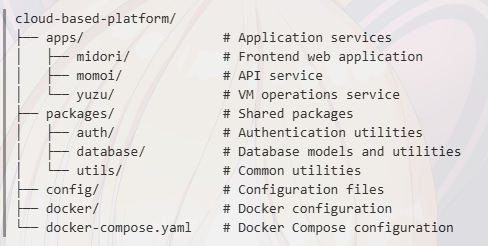
\includegraphics[width=0.8\textwidth]{Image/web/project_structure.png}
}
\caption{\fontSixTeen{โครงสร้างโปรเจกต์ทั้งหมด}}
\label{fig4:ProjectStructure}
\end{figure}

\hspace*{1.5em}
การจัดโครงสร้างโปรเจกต์ในลักษณะ Monorepo นี้ไม่เพียงแต่ช่วยให้โปรเจกต์เป็นระเบียบ แต่ยังช่วยลดความซับซ้อนในการจัดการ Dependencies ระหว่างแพ็กเกจ ทำให้การพัฒนาและการ Deploy เป็นทีมง่ายขึ้น และสามารถแชร์โค้ดระหว่างบริการต่าง ๆ ได้อย่างมีประสิทธิภาพ

\section{สถาปัตยกรรมระบบและเทคโนโลยี}
\subsection{การออกแบบสถาปัตยกรรมแบบ Microservices}
\hspace*{1.5em}
ระบบแพลตฟอร์มคลาวด์ที่พัฒนาขึ้นใช้สถาปัตยกรรมแบบ Microservices ซึ่งประกอบด้วยบริการหลัก 3 ตัว ที่ทำงานอิสระแต่สื่อสารกันผ่าน API และ Message Queue โดยแต่ละบริการมีหน้าที่และความรับผิดชอบที่แตกต่างกัน เพื่อให้ระบบมีความยืดหยุ่นและสามารถขยายตัวได้ง่าย

\hspace*{1.5em}
ภาพที่ \ref{fig4:SystemArchitecture} แสดงสถาปัตยกรรมระบบโดยรวม โดยมี \textbf{Midori} เป็นส่วนติดต่อผู้ใช้ที่พัฒนาด้วย Next.js และ Material UI \textbf{Momoi} เป็นบริการ API หลักที่จัดการการยืนยันตัวตน การจัดการผู้ใช้ และการเชื่อมต่อกับฐานข้อมูล และ \textbf{Yuzu} เป็นบริการจัดการเครื่องเสมือนที่เชื่อมต่อกับ Proxmox VE ผ่าน RabbitMQ

\begin{figure}[htbp]
\centering
\adjustbox{frame, width=0.9\textwidth}{
    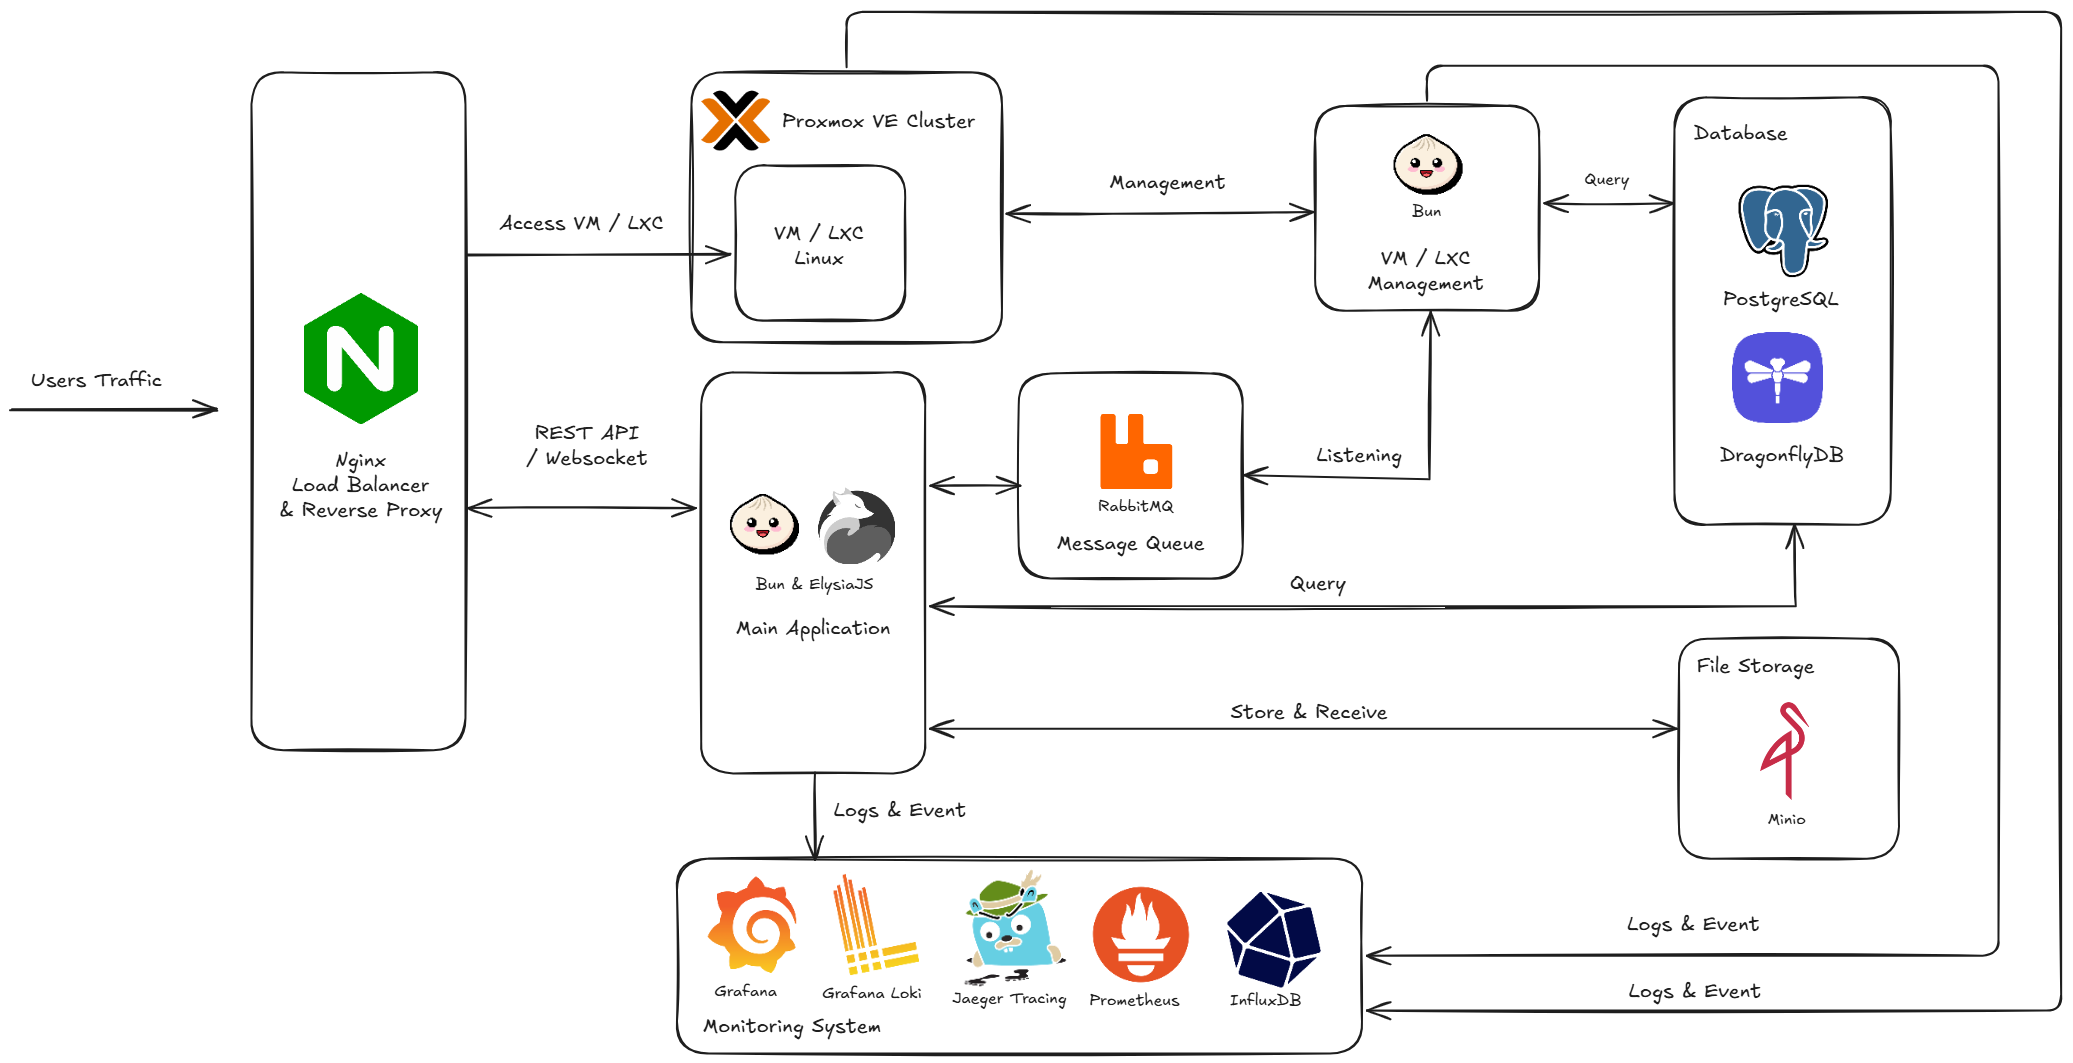
\includegraphics[width=0.9\textwidth]{Image/web/system_architecture.png}
}
\caption{\fontSixTeen{สถาปัตยกรรมระบบโดยรวม}}
\label{fig4:SystemArchitecture}
\end{figure}

\subsection{เทคโนโลยีที่ใช้ในการพัฒนา}
\hspace*{1.5em}
ในการพัฒนาระบบแพลตฟอร์มคลาวด์นี้ ได้เลือกใช้เทคโนโลยีที่ทันสมัยและเหมาะสมกับการใช้งานในสภาพแวดล้อมการศึกษา โดยเทคโนโลยีหลักที่ใช้ประกอบด้วย
\begin{mycustomitem}
    \item \textbf{Bun Runtime} - JavaScript/TypeScript Runtime ที่มีประสิทธิภาพสูง
    \item \textbf{Next.js} - React Framework สำหรับการพัฒนา Frontend
    \item \textbf{Elysia.js} - Web Framework สำหรับการพัฒนา API
    \item \textbf{PostgreSQL} - ระบบจัดการฐานข้อมูลเชิงสัมพันธ์
    \item \textbf{Prisma ORM} - Object-Relational Mapping สำหรับการจัดการฐานข้อมูล
    \item \textbf{RabbitMQ} - Message Queue สำหรับการสื่อสารระหว่างบริการ
    \item \textbf{Docker} - Container Platform สำหรับการ Deploy และการจัดการ Infrastructure
\end{mycustomitem}

\hspace*{1.5em}
การเลือกใช้เทคโนโลยีเหล่านี้มีเหตุผลสำคัญ คือ ความเสถียร ประสิทธิภาพ และการรองรับการขยายระบบในอนาคต รวมถึงการมี Community ที่ใหญ่และเอกสารประกอบที่ครบถ้วน ทำให้การพัฒนาและบำรุงรักษาระบบเป็นไปอย่างราบรื่น

\section{เอกสารประกอบการใช้งาน API และส่วนติดต่อผู้ใช้}
\subsection{เอกสาร API Documentation}
\hspace*{1.5em}
ระบบแพลตฟอร์มคลาวด์ได้จัดทำเอกสาร API Documentation อย่างครบถ้วนโดยใช้ OpenAPI Specification (Swagger) เพื่อให้ผู้พัฒนาและผู้ใช้งานสามารถเข้าใจและใช้งาน API ได้อย่างง่ายดาย เอกสารนี้ประกอบด้วยรายละเอียดของ Endpoints ต่าง ๆ พารามิเตอร์ที่ต้องการ รูปแบบข้อมูลที่ส่งและรับ รวมทั้งตัวอย่างการใช้งานที่ชัดเจน

\hspace*{1.5em}
ภาพที่ \ref{fig4:APIDocumentation} แสดงหน้าเอกสาร API Documentation ที่สร้างขึ้นโดยอัตโนมัติจากโค้ด TypeScript ผ่าน Elysia.js และ OpenAPI Plugin ซึ่งมีการจัดหมวดหมู่ API เป็นกลุ่มต่าง ๆ ดังนี้

\begin{mycustomitem}
    \item \textbf{Public API} - สำหรับการใช้งานทั่วไปที่ไม่ต้องมีการยืนยันตัวตน
    \item \textbf{Authentication API} - สำหรับการล็อกอิน ล็อกเอาต์ และการจัดการเซสชัน
    \item \textbf{Student API} - สำหรับนักศึกษาในการจัดการเครื่องเสมือนส่วนตัว
    \item \textbf{Staff API} - สำหรับอาจารย์และเจ้าหน้าที่ในการจัดการระบบ
    \item \textbf{Admin API} - สำหรับผู้ดูแลระบบในการจัดการผู้ใช้และทรัพยากร
\end{mycustomitem}

\begin{figure}[htbp]
\centering
\adjustbox{frame, width=0.9\textwidth}{
    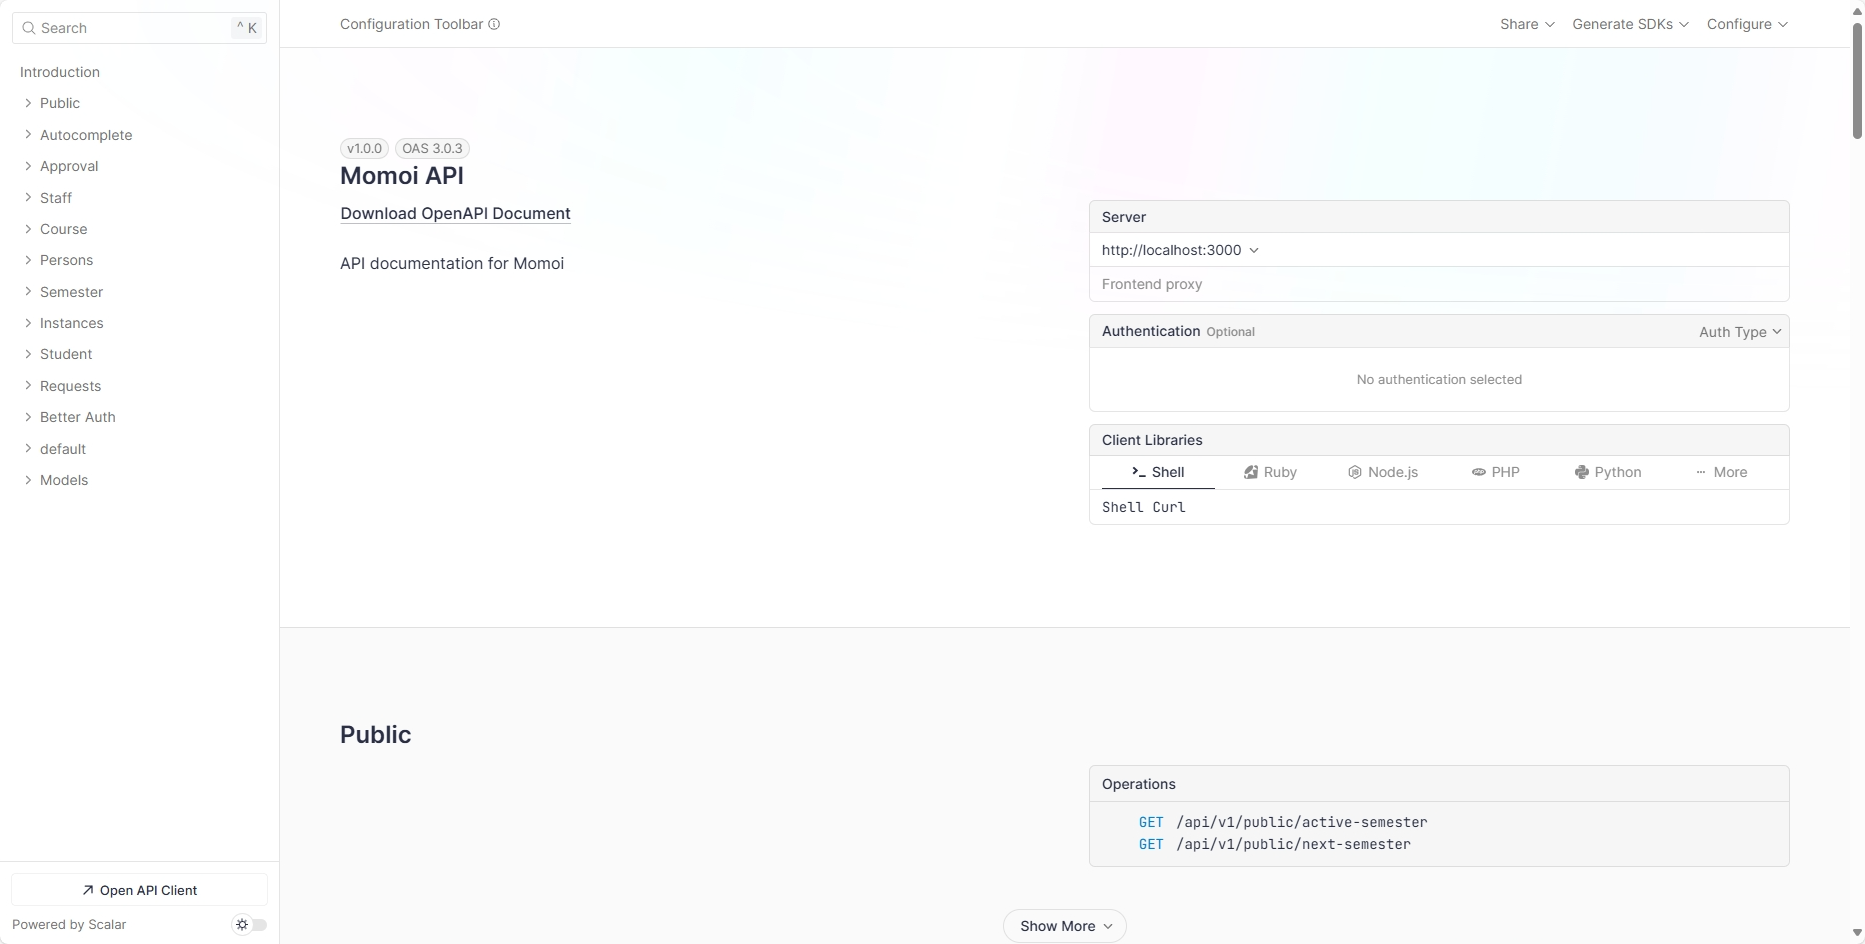
\includegraphics[width=0.9\textwidth]{Image/web/api_documentation.png}
}
\caption{\fontSixTeen{หน้าเอกสาร API Documentation}}
\label{fig4:APIDocumentation}
\end{figure}

\hspace*{1.5em}
เอกสาร API นี้มีการอัปเดตอัตโนมัติเมื่อมีการเปลี่ยนแปลงโค้ด และสามารถทดสอบ API ได้โดยตรงผ่านหน้าเว็บ ทำให้ผู้พัฒนาสามารถทำความเข้าใจและใช้งาน API ได้อย่างรวดเร็วและถูกต้อง

\subsection{ส่วนติดต่อผู้ใช้ (User Interface)}
\hspace*{1.5em}
ส่วนติดต่อผู้ใช้ของระบบได้รับการออกแบบให้ใช้งานง่าย สวยงาม และตอบสนองได้ดีบนอุปกรณ์ต่าง ๆ โดยใช้ Material UI และ Tailwind CSS ในการจัดรูปแบบ ระบบประกอบด้วยหน้าหลักต่าง ๆ ที่มีการจัดระเบียบข้อมูลและฟังก์ชันการทำงานอย่างชัดเจน

\hspace*{1.5em}
ภาพที่ \ref{fig4:LandingPage} แสดงหน้าแรกของระบบ (Landing Page) ที่ออกแบบให้ดึงดูดความสนใจและสื่อสารจุดประสงค์ของระบบได้ชัดเจน โดยมีการนำเสนอฟีเจอร์หลักของระบบ ข้อมูลการติดต่อ และลิงก์สำหรับการล็อกอินเข้าสู่ระบบ

\begin{figure}[htbp]
\centering
\adjustbox{frame, width=0.9\textwidth}{
    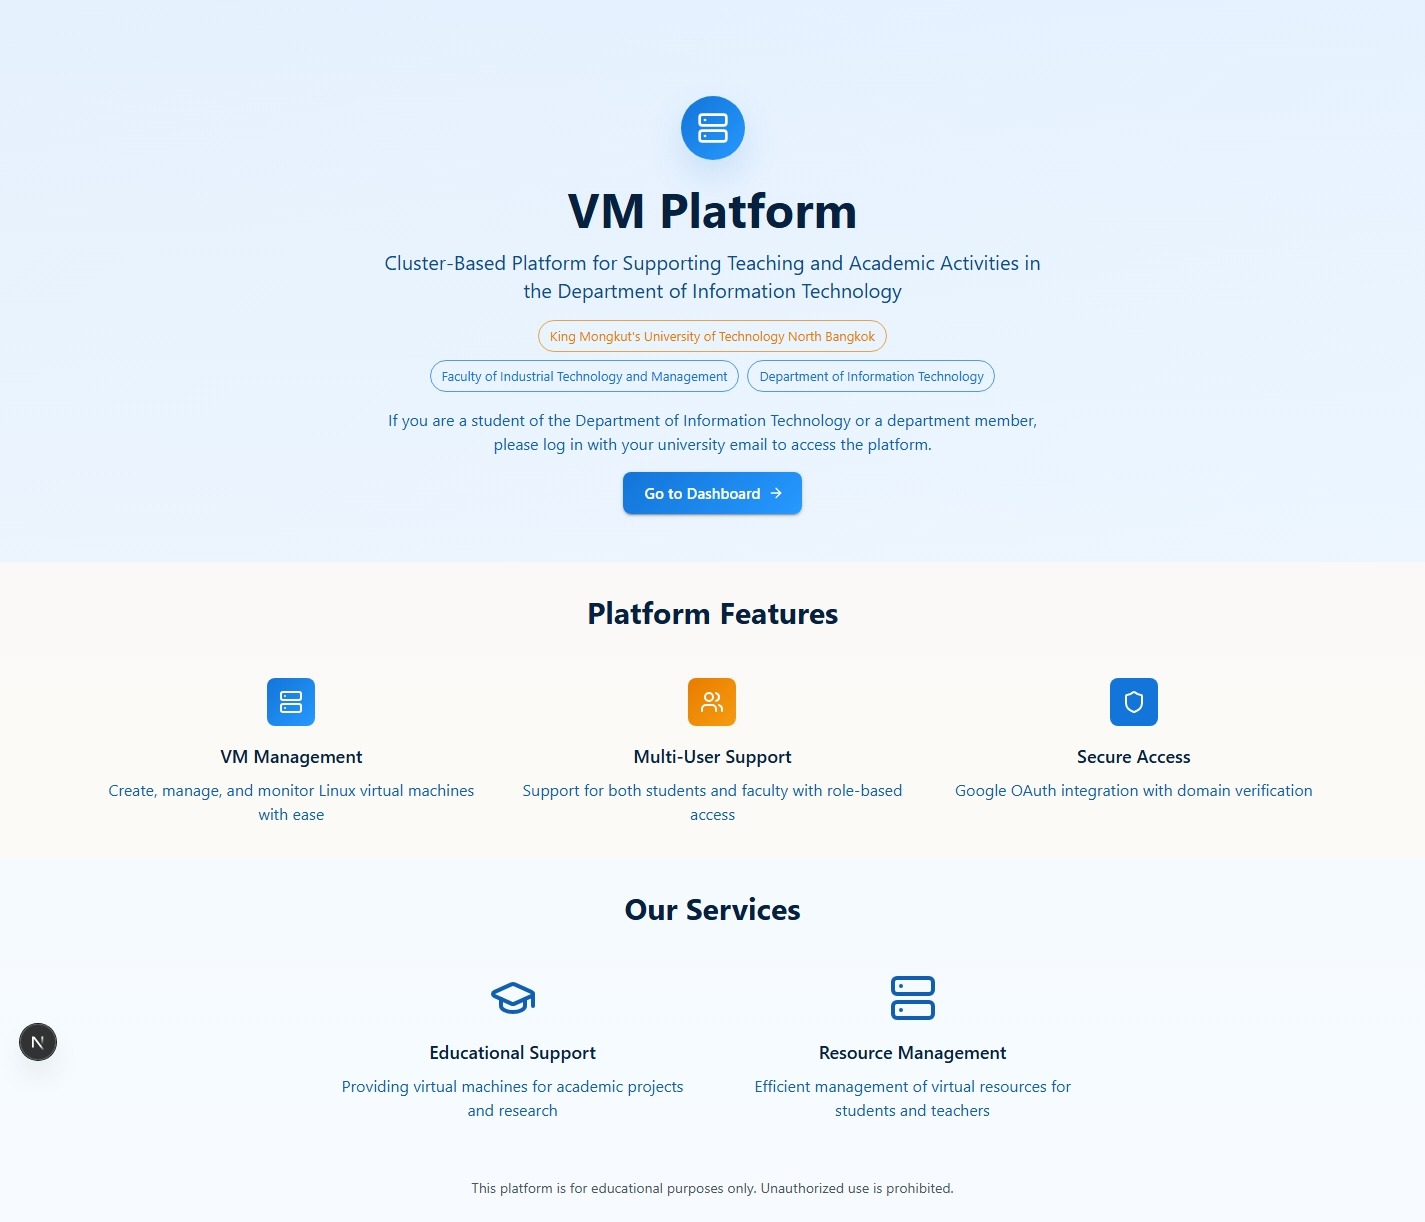
\includegraphics[width=0.9\textwidth]{Image/web/landing_page.jpeg}
}
\caption{\fontSixTeen{หน้าแรกของระบบ (Landing Page)}}
\label{fig4:LandingPage}
\end{figure}

\subsection{Dashboard และระบบจัดการ}
\hspace*{1.5em}
หลังจากที่ผู้ใช้ล็อกอินเข้าสู่ระบบแล้ว ผู้ใช้จะเข้าสู่หน้า Dashboard ที่แสดงข้อมูลสำคัญและฟังก์ชันการทำงานต่าง ๆ ตามบทบาทของผู้ใช้ โดย Dashboard ได้รับการออกแบบให้แสดงข้อมูลอย่างเป็นระบบและเข้าใจง่าย พร้อมทั้งมีการใช้งานที่สะดวกและรวดเร็ว

\hspace*{1.5em}
ส่วนติดต่อผู้ใช้ที่พัฒนาขึ้นมีลักษณะสำคัญดังนี้
\begin{mycustomitem}
    \item \textbf{Responsive Design} - รองรับการแสดงผลบนหน้าจอขนาดต่าง ๆ
    \item \textbf{Intuitive Navigation} - การนำทางที่เข้าใจง่ายและสอดคล้องกับมาตรฐาน UX
    \item \textbf{Real-time Updates} - การอัปเดตข้อมูลแบบเรียลไทม์
    \item \textbf{Accessibility} - การออกแบบที่คำนึงถึงผู้ใช้ที่มีความต้องการพิเศษ
    \item \textbf{Theme Support} - รองรับการเปลี่ยนธีมสีตามความต้องการ
\end{mycustomitem}

\hspace*{1.5em}
การออกแบบส่วนติดต่อผู้ใช้ได้คำนึงถึงประสบการณ์ผู้ใช้ (User Experience) เป็นหลัก โดยมุ่งเน้นให้ผู้ใช้สามารถทำงานได้อย่างมีประสิทธิภาพและลดข้อผิดพลาดในการใช้งาน ทั้งนี้ระบบยังมีการจัดการข้อผิดพลาดและการแจ้งเตือนที่ชัดเจน เพื่อให้ผู้ใช้สามารถแก้ไขปัญหาได้อย่างรวดเร็ว

\section{ตัวอย่างการใช้งานระบบตามบทบาทผู้ใช้}
\subsection{Dashboard สำหรับนักศึกษา}
\hspace*{1.5em}
ระบบได้จัดทำ Dashboard เฉพาะสำหรับนักศึกษา เพื่อให้สามารถจัดการเครื่องเสมือนส่วนตัวและติดตามการใช้งานทรัพยากรได้อย่างง่ายดาย ภาพที่ \ref{fig4:StudentDashboard} แสดง Dashboard หลักของนักศึกษาที่ประกอบด้วยข้อมูลสรุปการใช้งาน สถานะเครื่องเสมือน และฟังก์ชันการจัดการที่สำคัญ

\begin{figure}[htbp]
\centering
\adjustbox{frame, width=0.9\textwidth}{
    
\includegraphics[width=0.9\textwidth]{Image/web/dashboard/student/dashboard.jpeg}
}
\caption{\fontSixTeen{Dashboard หลักสำหรับนักศึกษา}}
\label{fig4:StudentDashboard}
\end{figure}

\hspace*{1.5em}
นักศึกษาสามารถดูรายการเครื่องเสมือนทั้งหมดที่ตนเองมีสิทธิ์เข้าถึง พร้อมทั้งสถานะการทำงาน การใช้ทรัพยากร และการจัดการพื้นฐาน ดังแสดงในภาพที่ \ref{fig4:StudentInstances} ซึ่งนำเสนอรายละเอียดของแต่ละ Instance อย่างชัดเจน

\begin{figure}[htbp]
\centering
\adjustbox{frame, width=0.9\textwidth}{
    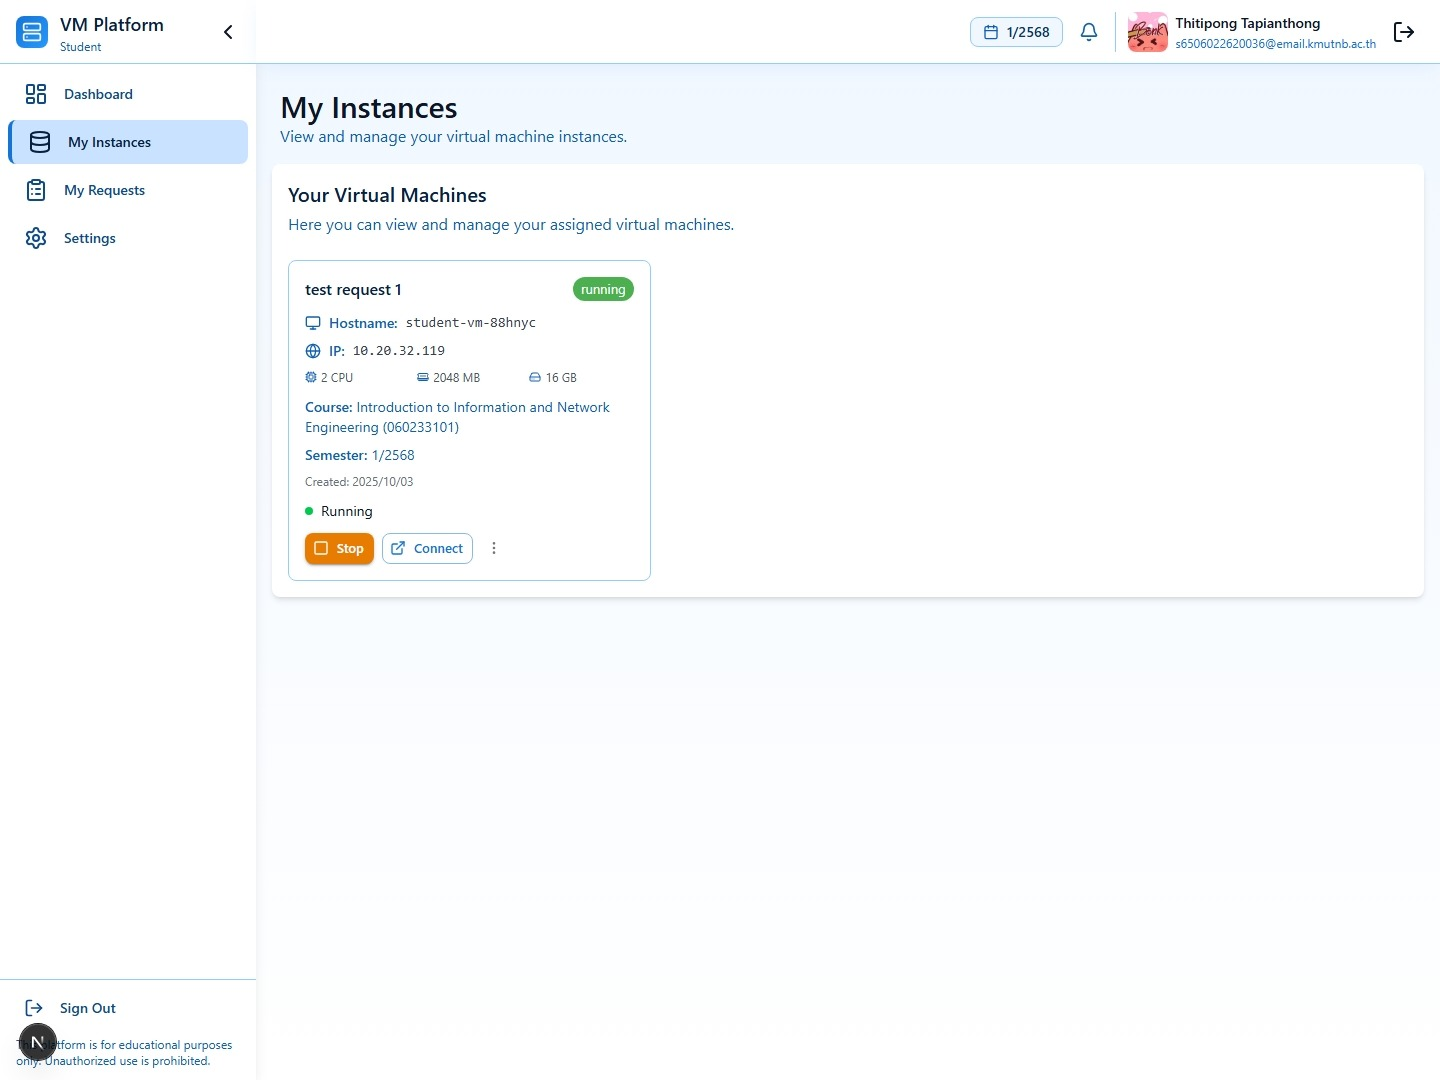
\includegraphics[width=0.9\textwidth]{Image/web/dashboard/student/instances.jpeg}
}
\caption{\fontSixTeen{หน้าจัดการ VM Instances สำหรับนักศึกษา}}
\label{fig4:StudentInstances}
\end{figure}

\subsection{Dashboard สำหรับอาจารย์และเจ้าหน้าที่}
\hspace*{1.5em}
สำหรับอาจารย์และเจ้าหน้าที่ ระบบได้จัดเตรียม Dashboard ที่มีฟังก์ชันการจัดการขั้นสูงมากขึ้น รวมถึงการอนุมัติคำขอ การจัดการหลักสูตร และการตรวจสอบการใช้งานของนักศึกษา ภาพที่ \ref{fig4:StaffDashboard} แสดง Dashboard หลักสำหรับเจ้าหน้าที่ที่มีข้อมูลสถิติและการควบคุมระบบ

\begin{figure}[htbp]
\centering
\adjustbox{frame, width=0.9\textwidth}{
    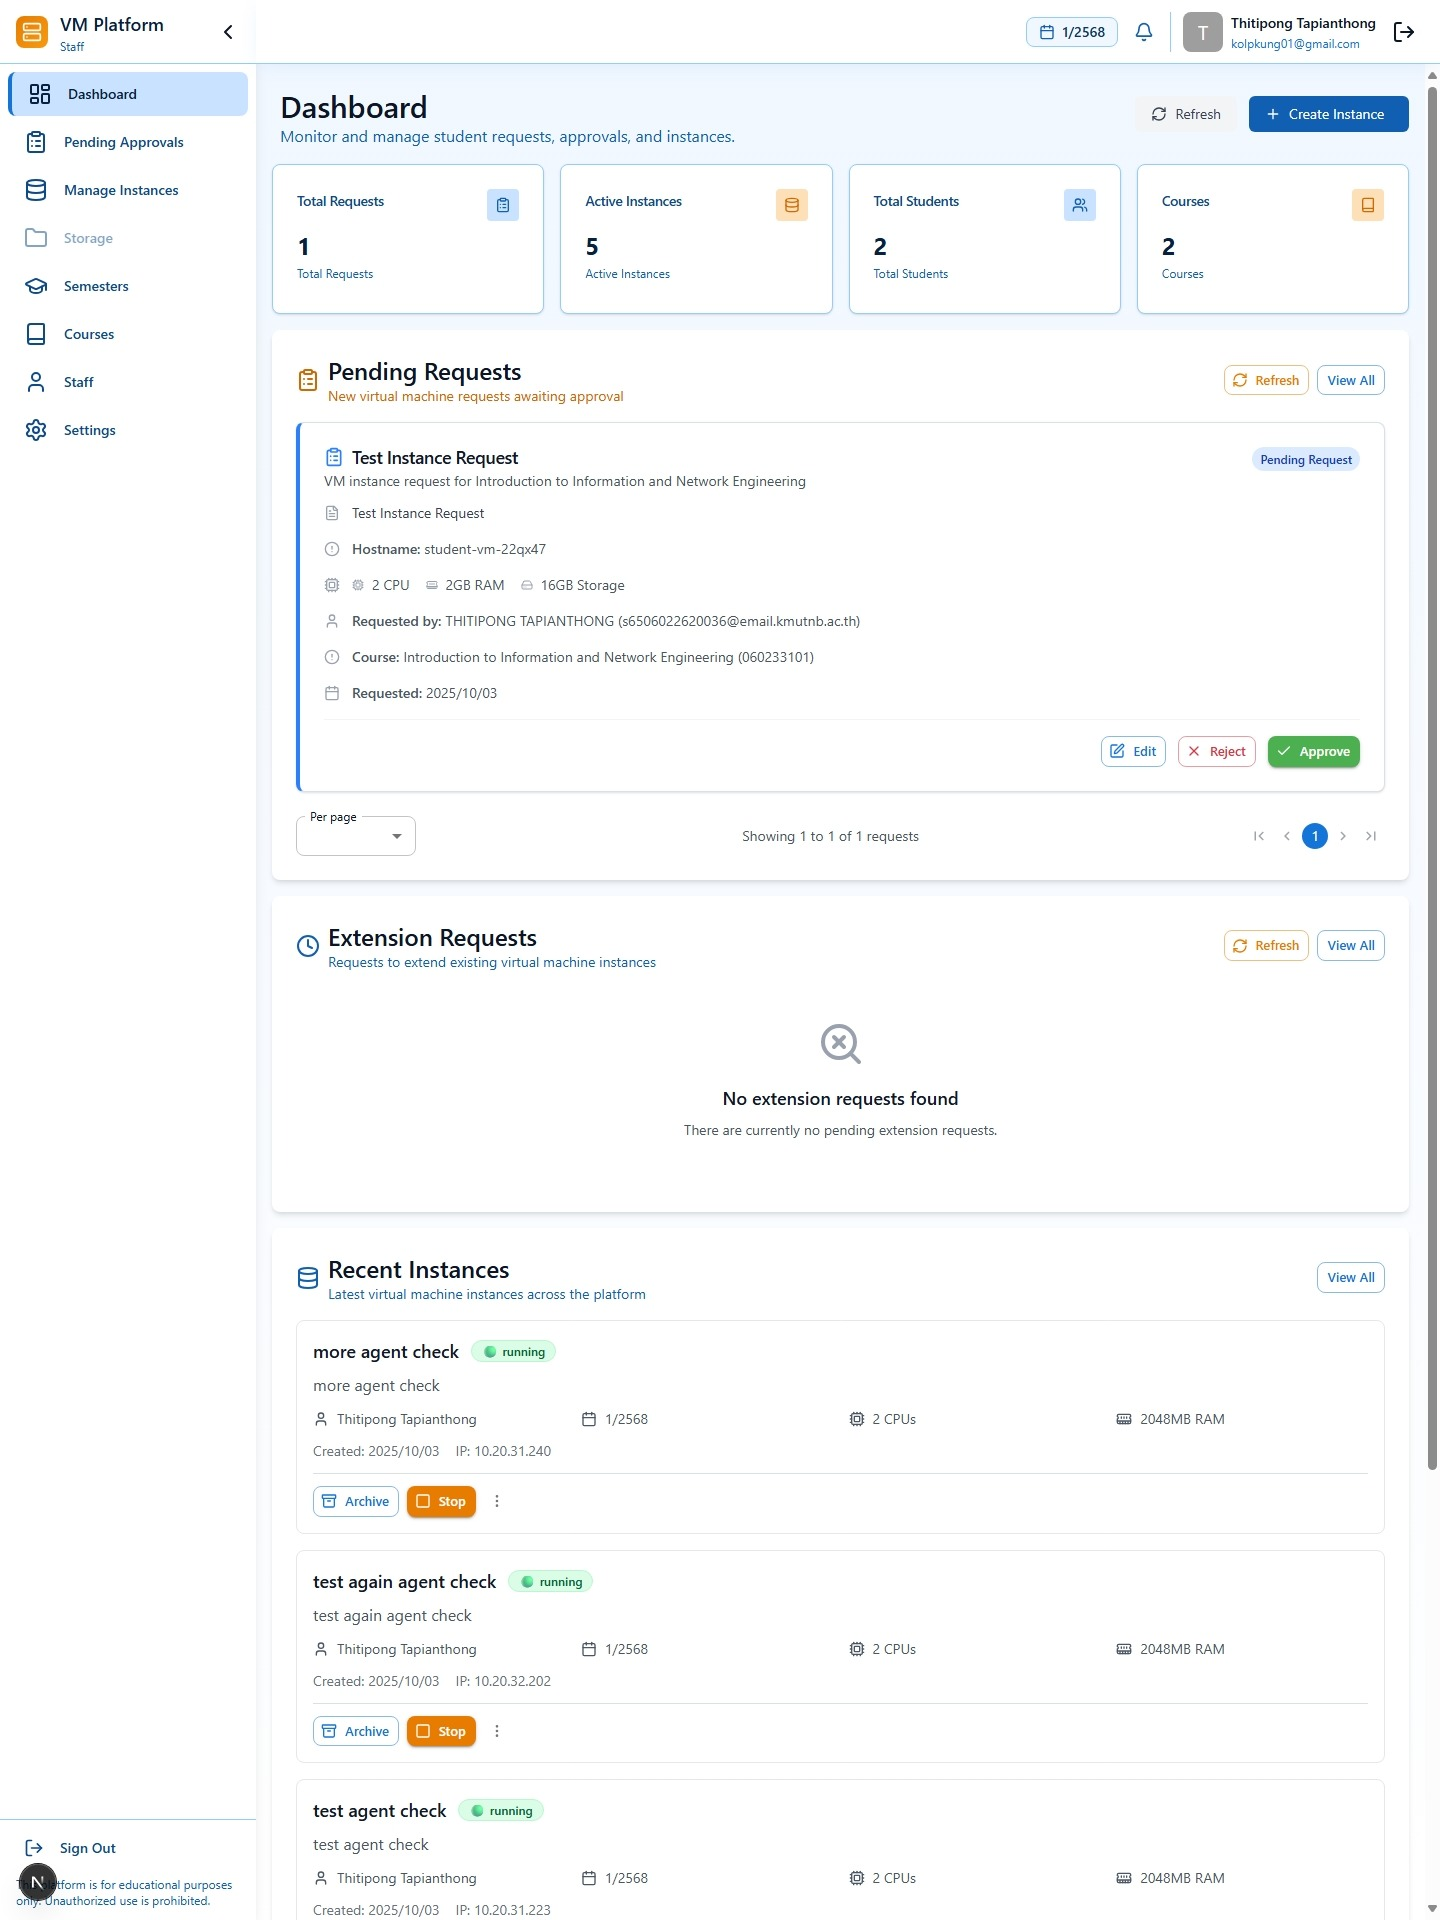
\includegraphics[width=0.9\textwidth]{Image/web/dashboard/staff/dashboard.jpeg}
}
\caption{\fontSixTeen{Dashboard หลักสำหรับอาจารย์และเจ้าหน้าที่}}
\label{fig4:StaffDashboard}
\end{figure}

\hspace*{1.5em}
อาจารย์และเจ้าหน้าที่สามารถจัดการหลักสูตรและเทอมการศึกษา ดังแสดงในภาพที่ \ref{fig4:CourseManagement} ซึ่งช่วยให้สามารถกำหนดทรัพยากรและสิทธิ์การเข้าถึงสำหรับแต่ละวิชาได้อย่างเหมาะสม

\begin{figure}[htbp]
\centering
\adjustbox{frame, width=0.9\textwidth}{
    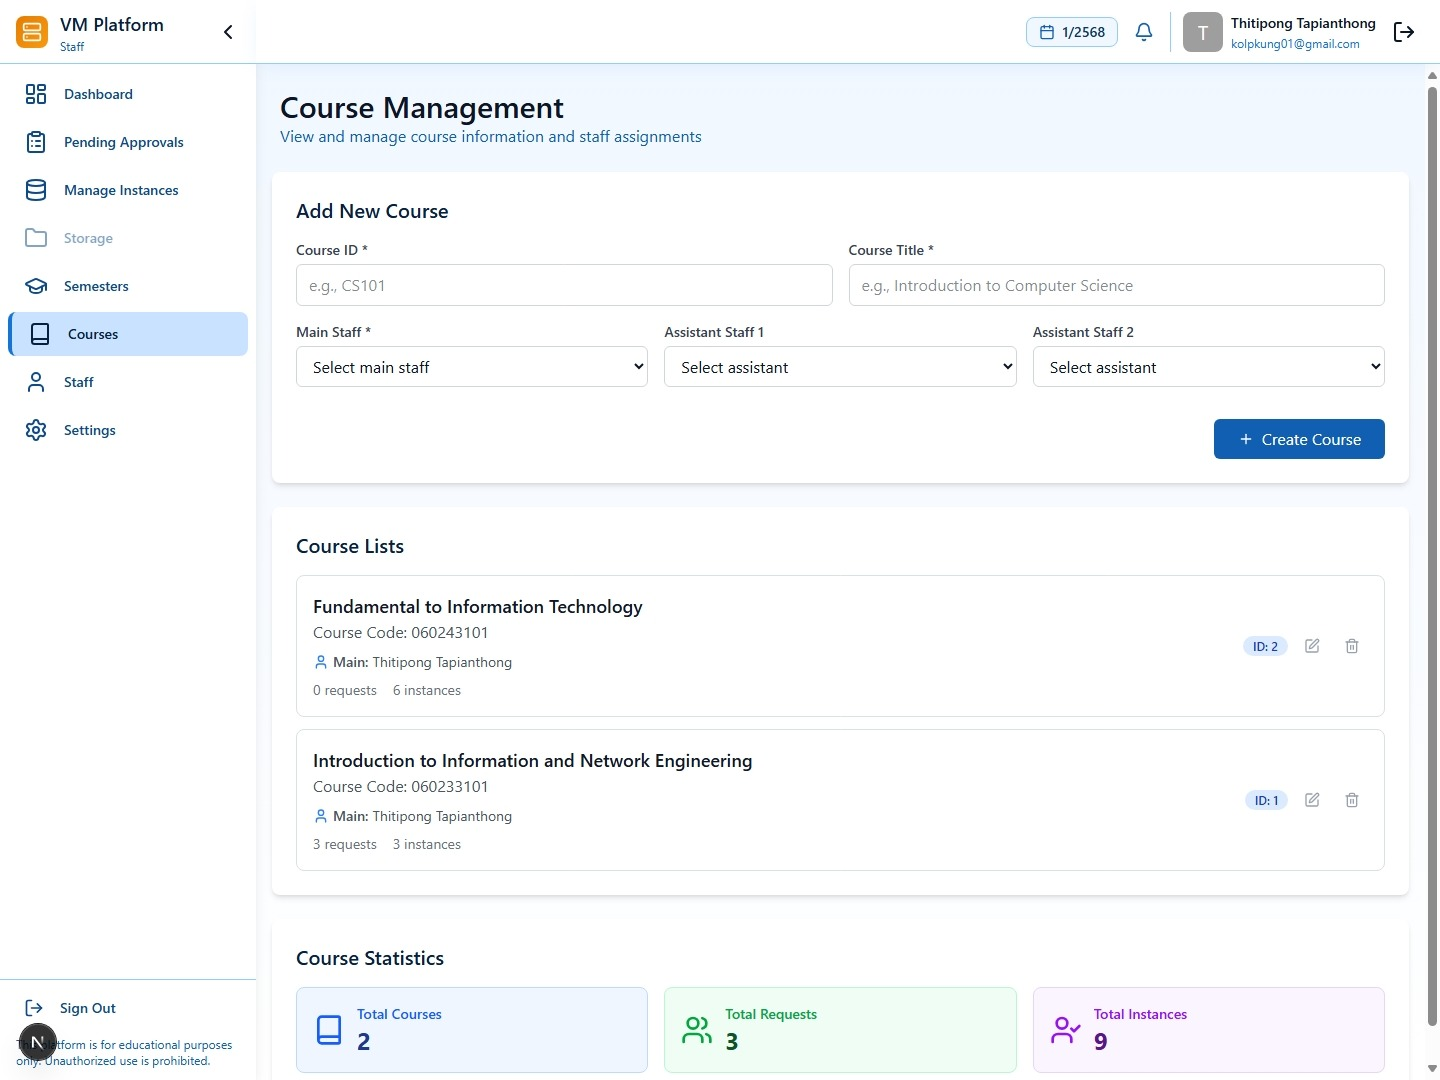
\includegraphics[width=0.9\textwidth]{Image/web/dashboard/staff/courses.jpeg}
}
\caption{\fontSixTeen{หน้าจัดการหลักสูตรและรายวิชา}}
\label{fig4:CourseManagement}
\end{figure}

\hspace*{1.5em}
นอกจากนี้ ระบบยังมีหน้าสำหรับการอนุมัติคำขอต่าง ๆ จากนักศึกษา ดังแสดงในภาพที่ \ref{fig4:PendingApproval} ซึ่งช่วยให้อาจารย์สามารถตรวจสอบและอนุมัติคำขอได้อย่างมีประสิทธิภาพ

\begin{figure}[htbp]
\centering
\adjustbox{frame, width=0.9\textwidth}{
    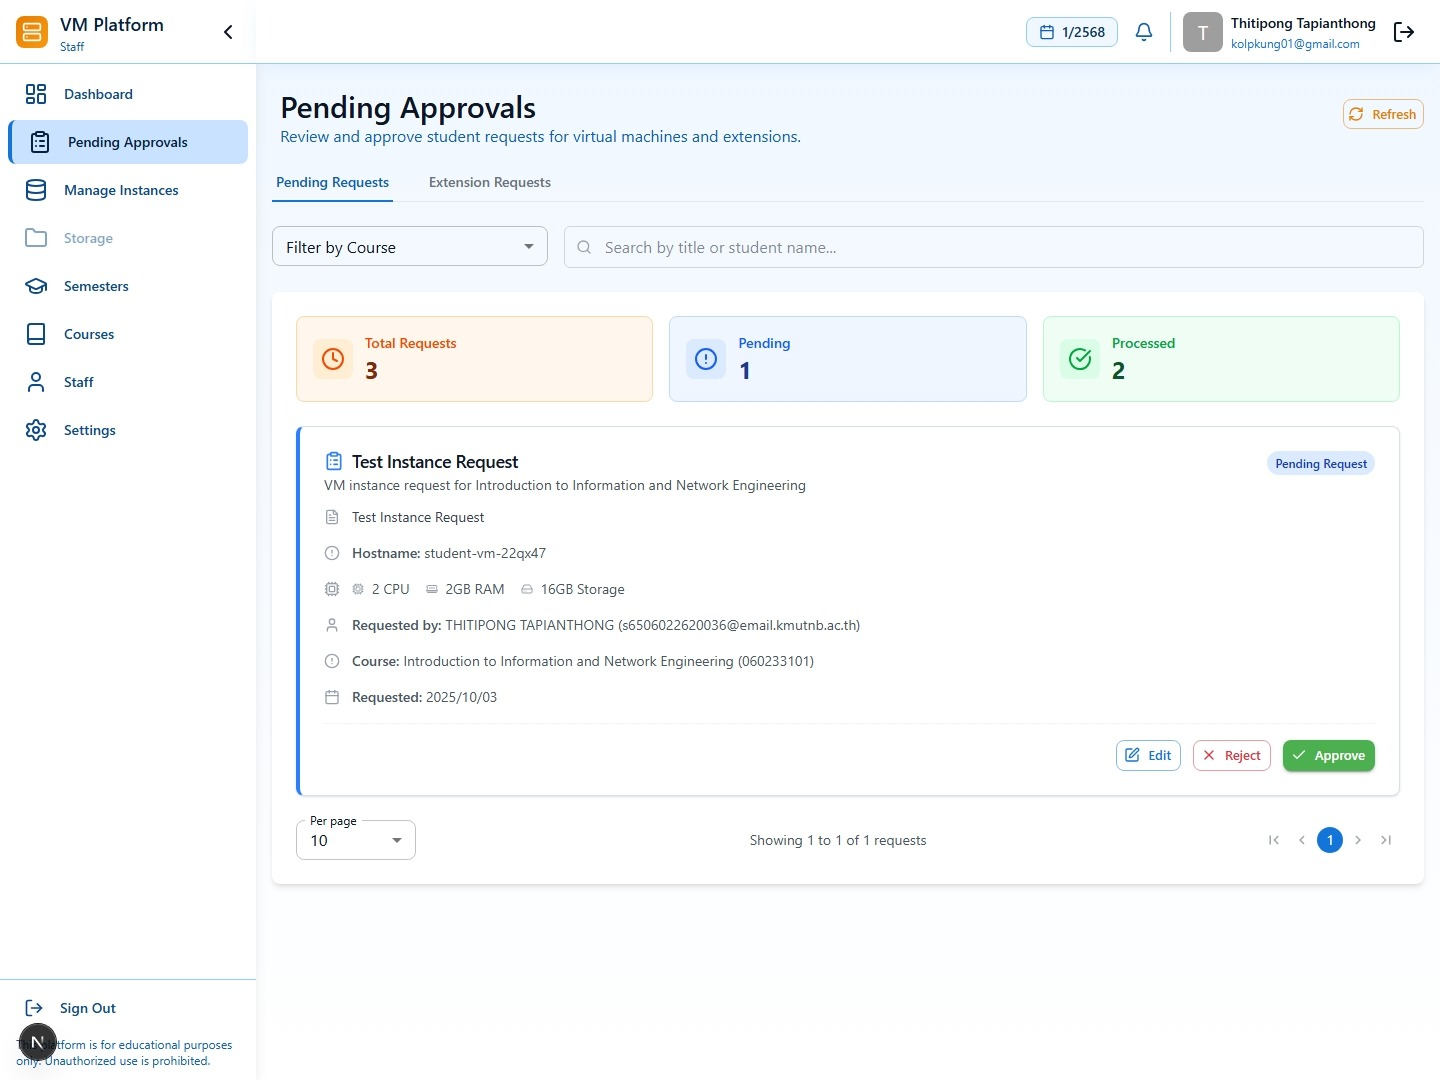
\includegraphics[width=0.9\textwidth]{Image/web/dashboard/staff/pending_approval.jpeg}
}
\caption{\fontSixTeen{หน้าอนุมัติคำขอที่รอดำเนินการ}}
\label{fig4:PendingApproval}
\end{figure}

\subsection{ระบบจัดการแบบ Role-Based Access Control}
\hspace*{1.5em}
ระบบได้นำเอา Role-Based Access Control (RBAC) มาใช้ในการจัดการสิทธิ์การเข้าถึงข้อมูลและฟังก์ชันต่าง ๆ โดยแบ่งผู้ใช้เป็น 3 กลุ่มหลัก คือ นักศึกษา อาจารย์ และผู้ดูแลระบบ ซึ่งแต่ละกลุ่มจะมีสิทธิ์และหน้าที่ที่แตกต่างกันตามความเหมาะสม

\hspace*{1.5em}
การออกแบบระบบในลักษณะนี้ช่วยให้การจัดการความปลอดภัยของข้อมูลเป็นไปอย่างมีประสิทธิภาพ และผู้ใช้แต่ละกลุ่มจะเห็นเฉพาะข้อมูลและฟังก์ชันที่เกี่ยวข้องกับหน้าที่ของตนเอง ทำให้การใช้งานง่ายขึ้นและลดความเสี่ยงในการเข้าถึงข้อมูลที่ไม่เหมาะสม
    \input{Project_050_Chapter5}

    \newgeometry{a4paper,top=1in,bottom=1in,left=1.5in,right=1in,includehead}
    \setTHSarabunFont
    \fontsize{16}{16}\selectfont
    \arabicPageTopRight
    \printbibliography[heading=mybibheading]
    \clearpage % ขึ้นหน้าใหม่หลังจากหน้าที่มีการปรับ margin
    \restoregeometry % คืนค่า geometry กลับเป็นค่าเริ่มต้น
    \fancyhf{} % ล้างการตั้งค่า fancyhdr ของหน้าที่ปรับ
    \setlength{\headsep}{0in}
    
    \appendixTitlePage
    % \input{Project_101_AppendixA}
    % \input{Project_102_AppendixB}
    \input{Project_103_AppendixC}
    % \input{Project_104_AppendixD}
    % \input{Project_105_AppendixE}

\end{document}
